\documentclass[t,12pt,numbers,fleqn]{beamer}
%\documentclass[t,12pt,numbers,fleqn,handout]{beamer}

\usepackage{latexsym}
\usepackage{amssymb}
\usepackage{stmaryrd}
\usepackage{phonetic}
\usepackage{wasysym}
\usepackage{pgf}
\usepackage{tikz}
\usepackage{url}
\usetikzlibrary{arrows}
\usepackage{array}
\usepackage{pgfpages} 
\usepackage{multirow} 
\usepackage{graphicx}
\usepackage{color}
\usepackage{listings}
\usepackage{hyperref}
\hypersetup{colorlinks=true,
    linkcolor=blue,
    citecolor=blue,
    filecolor=blue,
    urlcolor=blue,
    unicode=false}

\lstset{language=lisp,basicstyle=\ttfamily,breaklines=true,showspaces=false,showstringspaces=false,breakatwhitespace=true,texcl=true,escapeinside={\%*}{*)}}

%\pgfpagesuselayout{resize to}[letterpaper, border shrink=5mm,landscape] 
%\pgfpagesuselayout{2 on 1}[letterpaper,border shrink=5mm] 

\usepackage{fancybox}
%\usepackage{times}

\useoutertheme{split}

\mode<presentation>{}

%\mode<presentation>{
%\usecolortheme{whale}
%\usecolortheme{orchid}
%\useinnertheme[shadow]{rounded}
%}

%\setbeamerfont{structure}{series=\bfseries}
%\usefonttheme[stillsansseriftext,stillsansserifmath]{serif}
%\usetheme{Madrid}

\setbeamertemplate{navigation symbols}{} 
\setbeamertemplate{itemize item}[ball]
\setbeamersize{text margin left = 4mm}
\setbeamersize{text margin right = 4mm}

%% Requires:
%% 
%% \usepackage{latexsym}
%% \usepackage{amssymb}
%% \usepackage{stmaryrd}

%\renewcommand{\labelenumi}{(\theenumi)}
\newcommand{\be}{\begin{enumerate}}
\newcommand{\ee}{\end{enumerate}}
\newcommand{\bi}{\begin{itemize}}
\newcommand{\ei}{\end{itemize}}
\newcommand{\bc}{\begin{center}}
\newcommand{\ec}{\end{center}}
\newcommand{\bsp}{\begin{sloppypar}}
\newcommand{\esp}{\end{sloppypar}}

\newcommand{\sglsp}{\ }
\newcommand{\dblsp}{\ \ }

\newcommand{\iclicker}{i\texttt{>}clicker}

\newcommand{\sA}{\mbox{$\cal A$}}
\newcommand{\sB}{\mbox{$\cal B$}}
\newcommand{\sC}{\mbox{$\cal C$}}
\newcommand{\sD}{\mbox{$\cal D$}}
\newcommand{\sE}{\mbox{$\cal E$}}
\newcommand{\sF}{\mbox{$\cal F$}}
\newcommand{\sG}{\mbox{$\cal G$}}
\newcommand{\sH}{\mbox{$\cal H$}}
\newcommand{\sI}{\mbox{$\cal I$}}
\newcommand{\sJ}{\mbox{$\cal J$}}
\newcommand{\sK}{\mbox{$\cal K$}}
\newcommand{\sL}{\mbox{$\cal L$}}
\newcommand{\sM}{\mbox{$\cal M$}}
\newcommand{\sN}{\mbox{$\cal N$}}
\newcommand{\sO}{\mbox{$\cal O$}}
\newcommand{\sP}{\mbox{$\cal P$}}
\newcommand{\sQ}{\mbox{$\cal Q$}}
\newcommand{\sR}{\mbox{$\cal R$}}
\newcommand{\sS}{\mbox{$\cal S$}}
\newcommand{\sT}{\mbox{$\cal T$}}
\newcommand{\sU}{\mbox{$\cal U$}}
\newcommand{\sV}{\mbox{$\cal V$}}
\newcommand{\sW}{\mbox{$\cal W$}}
\newcommand{\sX}{\mbox{$\cal X$}}
\newcommand{\sY}{\mbox{$\cal Y$}}
\newcommand{\sZ}{\mbox{$\cal Z$}}

\renewcommand{\phi}{\varphi}
\newcommand{\seq}[1]{{\langle #1 \rangle}}
\newcommand{\set}[1]{{\{ #1 \}}}
\newcommand{\tuple}[1]{{( #1 )}}
\newcommand{\mlist}[1]{{[ #1 ]}}
\newcommand{\sembrack}[1]{\llbracket#1\rrbracket}
\newcommand{\redsembrack}[1]{\bred{\llbracket}#1\bred{\rrbracket}}
%\newcommand{\sembrack}[1]{[\![#1]\!]}
\newcommand{\synbrack}[1]{\ulcorner#1\urcorner}
\newcommand{\commabrack}[1]{\lfloor#1\rfloor}
\newcommand{\bsynbrack}[1]{\lceil#1\rceil}
\newcommand{\bsembrack}[1]{\lceil\!\!\lceil#1\rceil\!\!\rceil}
\newcommand{\mname}[1]{\mbox{\sf #1}}
\newcommand{\mcolon}{\mathrel:}
\newcommand{\mdot}{\mathrel.}
\newcommand{\modpar}{\models_{\rm par}}
\newcommand{\modreg}{\models_{\rm reg}}
\newcommand{\proves}[2]{#1 \vdash #2}
\newcommand{\notproves}[2]{#1 \not\vdash #2}
\newcommand{\provesin}[3]{#1 \vdash_{#2} #3}
\newcommand{\notprovesin}[3]{#1 \not\vdash_{#2} #3}
%\newcommand{\leqq}[1]{\mathrel{\preceq_{#1}}}
\newcommand{\parrow}{\rightharpoonup}
\newcommand{\tarrow}{\rightarrow}
\newcommand{\term}{\seq}
\newcommand{\lub}{\sqcup}
\newcommand{\subfun}{\sqsubseteq}
\newcommand{\subpred}{\subseteq}
\newcommand{\BoxApp}{\Box\,}
\newcommand{\BOX}{\mathrel{\Box}}
\newcommand{\funapp}{\mathrel@}

\newcommand{\com}{\mname{complement}}
\newcommand{\dom}{\mname{domain}}
\newcommand{\sumcl}{\mname{sum}}
\newcommand{\pow}{\mname{power}}
\newcommand{\pair}{\mname{pair}}
\newcommand{\opair}{\mname{ordered-pair}}
\newcommand{\inters}{\mname{intersection}}
\newcommand{\emp}{\mname{empty}}
\newcommand{\uni}{\mname{univocal}}
\newcommand{\fun}{\mname{function}}
\newcommand{\card}{\mname{card}}
\newcommand{\sets}{\mname{sets}}
\newcommand{\monotone}{\mname{monotone}}
\newcommand{\continuous}{\mname{continuous}}
\newcommand{\chain}{\mname{chain}}
\newcommand{\mub}{\mname{ub}}
\newcommand{\mlub}{\mname{lub}}
\newcommand{\fixedpoint}{\mname{fp}}
\newcommand{\leastfixedpoint}{\mname{lfp}}
\newcommand{\strongfixedpoint}{\mname{sfp}}
\newcommand{\emptyfun}{\triangle}
\newcommand{\statetrans}[1]{\stackrel{#1}{\longrightarrow}}
\newcommand{\thyext}{\leq}
\newcommand{\conthyext}{\unlhd}

\newcommand{\Iota}{\mbox{\rm I}}
\newcommand{\IotaApp}{\mbox{\rm I}\,}
\newcommand{\iotaApp}{\iota\,}
\newcommand{\epsilonApp}{\epsilon\,}
%\newcommand{\True}{\mbox{\sf T}} 
%\newcommand{\False}{\mbox{\sf F}} 
\newcommand{\Trueword}{\sf true}
\newcommand{\Falseword}{\sf false}
\newcommand{\Neg}{\neg} 
\newcommand{\Andd}{\wedge}
%\newcommand{\Or}{\vee}
\newcommand{\Orr}{\vee}
\newcommand{\Implies}{\supset}
\newcommand{\ImpliesAlt}{\Rightarrow}
\newcommand{\Iff}{\equiv}
\newcommand{\Sheffer}{\mathrel|}
\newcommand{\IffAlt}{\Leftrightarrow}
\newcommand{\Forall}{\forall}
\newcommand{\ForallApp}{\forall\,}
\newcommand{\Forsome}{\exists}
\newcommand{\ForsomeApp}{\exists\,}
\newcommand{\ForsomeUniqueApp}{\exists\,!\,}
\newcommand{\IsDef}{\downarrow}
\newcommand{\IsUndef}{\uparrow}
\newcommand{\Equal}{=}
\newcommand{\QuasiEqual}{\simeq}
\newcommand{\Undefined}{\bot}
\newcommand{\If}{\mname{if}}
\newcommand{\IsDefApp}{\!\IsDef}
\newcommand{\IsUndefApp}{\!\IsUndef}
\newcommand{\TRUE}{\mbox{{\sc t}}}
\newcommand{\FALSE}{\mbox{{\sc f}}}
\newcommand{\truthvalues}{\{\TRUE,\FALSE\}}
\newcommand{\LambdaApp}{\lambda\,}
\newcommand{\LAMBDAapp}{\Lambda\,}
\newcommand{\PiApp}{\Pi\,}
\newcommand{\SigmaApp}{\Sigma\,}
\newcommand{\AlphaEquiv}{\stackrel{\alpha}{=}}

\newcommand{\mvar}[3]{\textbf{var}_{#1}[#2,#3]}
\newcommand{\mterm}[2]{\textbf{term}_{#1}[#2]}
\newcommand{\mform}[2]{\textbf{form}_{#1}[#2]}
\newcommand{\mtype}[2]{\textbf{type}_{#1}[#2]}
\newcommand{\mexpr}[3]{\textbf{expr}_{#1}[#2,#3]}

\newcommand{\imps}{\mbox{\sc imps}}
\newcommand{\fol}{\mbox{\sc fol}}
\newcommand{\pf}{${\bf PF}$}
\newcommand{\pfstar}{${\bf PF}^\ast$}
\newcommand{\lutins}{\mbox{\sc lutins}}
\newcommand{\vlisp}{\mbox{\sc vlisp}}
\newcommand{\vmach}{\mbox{\sc vmach}}
\newcommand{\gnu}{\mbox{\sc gnu}}
\newcommand{\zf}{\mbox{\sc zf}}
\newcommand{\nbg}{\mbox{\sc nbg}}
\newcommand{\pnbg}{\mbox{\sc pnbg}}
\newcommand{\snbg}{\mbox{\sc snbg}}
\newcommand{\pfol}{\mbox{\sc pfol}}
\newcommand{\nbgstar}{$\mbox{\sc nbg}^\ast$}
\newcommand{\boldnbgstar}{$\mbox{\bf NBG}^\ast$}
\newcommand{\stt}{\mbox{\sc stt}}
\newcommand{\eves}{\mbox{\sc eves}}
\newcommand{\hol}{\mbox{\sc hol}}
\newcommand{\mizar}{Mizar}
\newcommand{\nqthm}{Nqthm}
\newcommand{\pvs}{\mbox{\sc pvs}}
\newcommand{\stmm}{\mbox{\sc stmm}}

\iffalse
\newtheorem{thm}{Theorem}[section]
\newtheorem{cor}[thm]{Corollary}
\newtheorem{lem}[thm]{Lemma}
\newtheorem{prop}[thm]{Proposition}
\newtheorem{rem}[thm]{Remark}
\newtheorem{eg}[thm]{Example}
\newtheorem{df}[thm]{Definition}
\fi

%\newenvironment{proof}{\par\noindent{\bf Proof\ \ }}{$\Box$}

\newenvironment{namedform}[1]
   {\begin{tabbing}\textbf{#1}\ }
   {\end{tabbing}}

\newcommand{\urlpart}[1]{\mbox{\texttt{#1}}\linebreak[0]}

\newcommand{\bblue}{\textcolor{blue!80!black}}
\newcommand{\bgreen}{\textcolor{green!55!black}}
\newcommand{\bbrown}{\textcolor{brown}}
\newcommand{\bred}{\textcolor{red!80!black}}
\newcommand{\bcyan}{\textcolor{cyan!80!black}}
\newcommand{\bmagenta}{\textcolor{magenta}}
\newcommand{\byellow}{\textcolor{yellow}}
\newcommand{\borange}{\textcolor{orange}}
\newcommand{\bviolet}{\textcolor{violet}}
\newcommand{\bpurple}{\textcolor{purple}}
\newcommand{\bdarkgray}{\textcolor{darkgray}}
\newcommand{\bgray}{\textcolor{gray}}
\newcommand{\blightgray}{\textcolor{lightgray}}

\newcommand{\clicker}{i\texttt{>}clicker}

\newenvironment{changemargin}[2]{%
  \begin{list}{}{%
    \setlength{\topsep}{0pt}%
    \setlength{\leftmargin}{#1}%
    \setlength{\rightmargin}{#2}%
    \setlength{\listparindent}{\parindent}%
    \setlength{\itemindent}{\parindent}%
    \setlength{\parsep}{\parskip}%
  }%
  \item[]}{\end{list}}


\newcommand{\qzero}{${\cal Q}_0$}
\newcommand{\qzerou}{${\cal Q}^{\rm u}_{0}$}
\newcommand{\qzerouqe}{${\cal Q}^{\rm uqe}_{0}$}
\newcommand{\churchqe}{$\mbox{\sc ctt}_{\rm qe}$}
\newcommand{\churchuqe}{$\mbox{\sc ctt}_{\rm uqe}$}
\newcommand{\NegAlt}{{\sim}}
\newcommand{\wff}[1]{{\sf wff}_{#1}}
\newcommand{\additionu}[1]{\textcolor{blue}{#1}}
\newcommand{\additionuqe}[1]{\textcolor{red}{#1}}

\newcommand{\high}{\bred{\rotatebox[origin=c]{90}{\CIRCLE}}}
\newcommand{\medhigh}{\bred{\rotatebox[origin=c]{90}{\RIGHTcircle}}}
\newcommand{\medlow}{\bred{\rotatebox[origin=c]{-90}{\RIGHTcircle}}}
\newcommand{\low}{\bred{\rotatebox[origin=c]{90}{\Circle}}}


\title{ {\normalsize \bgreen{\bf ITP 2018}}\\[1.5ex]
  {\large \bf HOL Light QE}
\vspace{-1.5ex}
}

\author[Farmer]{
Jacques Carette, \underline{William M. Farmer}, and Patrick Laskowski\\
\vspace*{-1.5ex}
}

\institute{
Department of Computing and Software\\
McMaster University
\vspace*{-1.5ex}
} 

\date{
{\small 11 July 2018}

\bc
 \includegraphics[scale = 0.2, keepaspectratio]
{$HOME/doc/images/mcmaster-logo-full-color.jpg}%$
\ec
}

\begin{document}

%%%%%%%%%%%%%%%%%%%%%%%%%%%%%%%%%%%%%%%%%%%%%%%%%%%%%%%%%%%%

\setbeamertemplate{footline}{}
\begin{frame}
\vspace{-1.5ex} 
\titlepage
\end{frame}

\setbeamertemplate{footline}{
\begin{beamercolorbox}{sectioninhead/foot}
\bblue{\hrulefill}

\vspace{1ex}
\hspace{1ex}
{\tiny W. M. Farmer
\hfill 
HOL Light QE
\hfill
\insertframenumber/\ref{lastframe}}
\vspace{1ex}
\end{beamercolorbox}}

%%%%%%%%%%%%%%%%%%%%%%%%%%%%%%%%%%%%%%%%%%%%%%%%%%%%%%%%%%%%

\begin{frame}
\frametitle{Outline}
\bi

  \item Syntax-based mathematical algorithms.

  \item Local and global reflection.

  \item {\churchqe}, Church's type theory with quotation and
    evaluation.

  \item HOL Light QE, an implementation of {\churchqe}.

\ei
\end{frame}

%%%%%%%%%%%%%%%%%%%%%%%%%%%%%%%%%%%%%%%%%%%%%%%%%%%%%%%%%%%%

\begin{frame}
\frametitle{A Warm-Up Example}
\bi

  \item \bgreen{Problem}: Are the following two functions equal?

  \bi

    \item[] \only<1>{$\LambdaApp x \mcolon \mathbb{R} \mdot (x + 2) *
      (2 * x + 1) + 3 * x$}
    
    \only<2->{$\LambdaApp x \mcolon \mathbb{R} \mdot
      \colorbox{yellow!40}{$(x + 2) * (2 * x + 1) + 3 * x$}$}

    \item[] \only<1>{$\LambdaApp x \mcolon \mathbb{R} \mdot 2 * (x +
      2)^2 - 6$}

    \only<2->{$\LambdaApp x \mcolon \mathbb{R} \mdot
      \colorbox{brown!40}{$2 * (x + 2)^2 - 6$}$} 

  \ei 

  \only<2->{\bred{Notice the polynomials.}}

  \item<3-> \bgreen{Solution}: Normalize the polynomial 

  \bi

    \item[] $\colorbox{yellow!40}{$((x + 2) * (2 * x + 1) + 3 * x)$} -
      \colorbox{brown!40}{$(2* (x + 2)^2 - 6)$}$

  \ei

  and see if it is the 0 polynomial.

\pause

  \item<4-> \bblue{``normalize''} is an algorithm that:

  \be

    \item Manipulates mathematical expressions having the form of
      polynomials.

    \item Preserves the mathematical meaning of the expressions.

  \ee

\ei
\end{frame}

%%%%%%%%%%%%%%%%%%%%%%%%%%%%%%%%%%%%%%%%%%%%%%%%%%%%%%%%%%%%

\begin{frame}
\frametitle{Syntax-Based Mathematical Algorithms}
\bi

  \item A \bblue{syntax-based mathematical algorithm (SBMA)} is an
    algorithm that manipulates the syntax of mathematical
    expressions in a mathematically meaningful way.

\pause

  \bi

    \item SBMAs are commonplace in mathematics.

    \item ``normalize'' is an example.

  \ei

\pause

  \item A SBMA $A$ has two fundamental properties:

  \be

    \item The \bblue{computational behavior} of $A$ is the relationship
    between the input and output expressions of $A$.

    \item The \bblue{mathematical meaning} of $A$ is the relationship
      between what the input and output expressions of $A$ mean
      mathematically.

  \ee

\pause

  \item A \bblue{meaning formula} for $A$ is a statement that
    expresses the mathematical meaning of $A$.

\ei
\end{frame}

%%%%%%%%%%%%%%%%%%%%%%%%%%%%%%%%%%%%%%%%%%%%%%%%%%%%%%%%%%%%

\begin{frame}
\frametitle{Example: Meaning Formula for ``normalize''}
\bi

  \item<1-> $\mname{normalize} : \mname{Poly} \tarrow \mname{Poly}$

  \medskip

  \item<2->[]

  \only<2>{
  $\ForallApp p,q \mcolon \mname{Poly} \mdot$\\
  \hspace{2ex}$(\ForallApp x \mcolon \mathbb{R} \mdot 
  p = \mname{normalize}(p)) \Andd {}$\\
  \hspace{2ex}$(\ForallApp x \mcolon \mathbb{R} \mdot
  p = q) \Iff \mname{normalize}(p) = \mname{normalize}(q)$
  }

  \only<3>{
  $\ForallApp \colorbox{yellow!40}{p},\colorbox{yellow!40}{q} \mcolon \mname{Poly} \mdot$\\
  \hspace{2ex}$(\ForallApp x \mcolon \mathbb{R} \mdot 
  \colorbox{yellow!40}{p} = \colorbox{yellow!40}{\mname{normalize}(p)}) \Andd {}$\\
  \hspace{2ex}$(\ForallApp x \mcolon \mathbb{R} \mdot
  \colorbox{yellow!40}{p} = \colorbox{yellow!40}{q}) \Iff 
  \colorbox{yellow!40}{\mname{normalize}(p)} = \colorbox{yellow!40}{\mname{normalize}(q)}$
  }

  \only<4>{
  $\ForallApp \colorbox{yellow!40}{p},\colorbox{yellow!40}{q} \mcolon \mname{Poly} \mdot$\\
  \hspace{2ex}$(\ForallApp x \mcolon \mathbb{R} \mdot 
  \colorbox{cyan}{\colorbox{yellow!40}{p}} = 
  \colorbox{cyan}{\colorbox{yellow!40}{\mname{normalize}(p)}}) \Andd {}$\\
  \hspace{2ex}$(\ForallApp x \mcolon \mathbb{R} \mdot
  \colorbox{cyan}{\colorbox{yellow!40}{p}} = \colorbox{cyan}{\colorbox{yellow!40}{q}}) \Iff 
  \colorbox{yellow!40}{\mname{normalize}(p)} = \colorbox{yellow!40}{\mname{normalize}(q)}$
  }

  \only<5->{
  $\ForallApp p,q \mcolon \mname{Poly} \mdot$\\
  \hspace{2ex}$(\ForallApp x \mcolon \mathbb{R} \mdot 
  \redsembrack{p} = \redsembrack{\mname{standardize}(p)}) \Andd {}$\\
  \hspace{2ex}$(\ForallApp x \mcolon \mathbb{R} \mdot
  \redsembrack{p} = \redsembrack{q}) \Iff 
  \mname{standardize}(p) = \mname{standardize}(q)$
  }

\bigskip

  \only<5->{$\redsembrack{\cdot}$ is the \bgreen{evaluation operator}.}

\medskip

  \item<6-> The required result is obtained by instantiating $p$ and
    $q$ with

  \bi

    \item[] $\redsynbrack{(x + 2) * (2 * x + 1) + 3 * x}$ 

  \ei

  and

  \bi

    \item[] $\redsynbrack{2 * (x + 2)^2 - 6}$.

  \ei

\medskip

  $\redsynbrack{\cdot}$ is the \bgreen{quotation operator}.

\ei
\end{frame}

%%%%%%%%%%%%%%%%%%%%%%%%%%%%%%%%%%%%%%%%%%%%%%%%%%%%%%%%%%%%

\begin{frame}
\frametitle{Quotation and Evaluation}
\bi

  \item \bblue{Quotation} is used to gain access to the
    \bgreen{syntax} of an expression.

  \bi

    \item The value of \bred{$\synbrack{e}$} is a \bblue{syntactic
      value} that represents the syntactic structure of the expression
      \bred{$e$}.

    \item Note: $\bred{\synbrack{2 + 3}} \not= \bred{\synbrack{5}}$.

  \ei

\pause
\medskip

  \item \bblue{Evaluation} is used to obtain the \bgreen{semantics} of
    the expression represented by a syntactic value.

  \bi

    \item If the value of \bred{$e'$} is a syntactic value \bred{$e$},
      then the value of \bred{$\sembrack{e'}$} is the value of
      \bred{$e$}.

  \ei

\pause
\medskip

  \item The two operators are related by the \bblue{law of disquotation}:

  \bi

    \item[] \bred{$\sembrack{\synbrack{e}} = e$}.

  \ei

\ei
\end{frame}

%%%%%%%%%%%%%%%%%%%%%%%%%%%%%%%%%%%%%%%%%%%%%%%%%%%%%%%%%%%%

\begin{frame}
\frametitle{Formalizing SBMAs}
\bi

  \item To employ an SBMA $A$ in a \bgreen{proof assistant} (or
    other \bgreen{formal environment}) we need to formalize $A$
    in the \bgreen{logic} of the system.

\bigskip

  \item To formalize an SBMA $A$ in a logic Log we need
    to be able to:

  \be

    \item Define in Log a function $B$ on syntactic
      values representing $A$.

    \item State and prove in Log the meaning formula for
      $B$ from the definition of $B$.

    \item Apply $B$ to mathematical expressions in Log by
      instantiating the meaning formula for $B$ and then simplifying.

  \ee

\ei
\end{frame}

%%%%%%%%%%%%%%%%%%%%%%%%%%%%%%%%%%%%%%%%%%%%%%%%%%%%%%%%%%%%

\begin{frame}
\frametitle{Standard Approach: Local Reflection}
\bi

  \item Let $A$ be an SBMA on expressions in a language $L_{\rm obj}$
    of some logic Log.

  \item We build a \bblue{metareasoning infrastructure} in Log
    consisting of:

  \be

    \item An \bgreen{inductive type} $L_{\rm syn}$ of syntactic values
      representing the expressions in $L_{\rm obj}$.

    \item A \bgreen{quotation operator} $\synbrack{\cdot}$ mapping
      expressions in $L_{\rm obj}$ to syntactic values of $L_{\rm
        syn}$.

    \item An \bgreen{evaluation operator} $\sembrack{\cdot}$
      mapping syntactic values of $L_{\rm syn}$ to values of $L_{\rm
        obj}$.

  \ee

  \item We define a function $B$ in Log from
    syntactic values representing inputs of $A$ to syntactic
    values representing outputs of $A$.

  \item The infrastructure is \bgreen{local} in the sense that $L_{\rm
    obj}$ is not the whole language $L$ of Log.

\ei
\end{frame}

%%%%%%%%%%%%%%%%%%%%%%%%%%%%%%%%%%%%%%%%%%%%%%%%%%%%%%%%%%%%

\begin{frame}
\frametitle{Local Reflection}
\vspace*{-3ex}
\vfill
\begin{figure}
\center
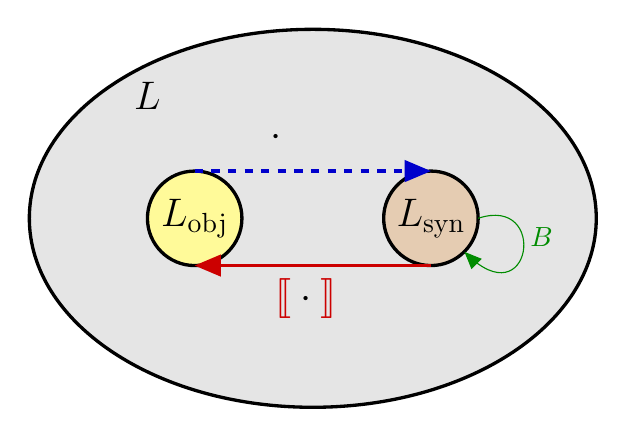
\begin{tikzpicture}[scale=.6]
  \filldraw[very thick, fill=gray!20] (3.5,0) ellipse (6 and 4);
    \draw (0,+2.6) node {\Large $L$};
  \filldraw[very thick, fill=yellow!40] (+1,0) circle (1);
    \draw (+1,0) node {\Large $L_{\rm obj}$};
  \filldraw[very thick, fill=brown!40] (+6,0) circle (1);
    \draw (+6,0) node {\Large $L_{\rm syn}$};
  \draw[-triangle 45, very thick, dashed, color=blue!80!black] (+1,+1) -- (+6,+1);
    \draw[right] (+2.4,+1.7) node {\Large $\bluesynbrack{\cdot}$};
  \draw[-triangle 45, very thick, color=red!80!black] (+6,-1) -- (+1,-1);
    \draw[right] (+2.5,-1.7) node {\Large $\redsembrack{\cdot}$};
  \draw[-triangle 45, color=green!55!black] (7,0) .. controls 
    (8.5,.5) and (8.13,-2.13) .. (6.71,-.71);
    \draw[right] (7.9,-.4) node {\bgreen{$B$}};
\end{tikzpicture}
\end{figure}
\vfill
\end{frame}

%%%%%%%%%%%%%%%%%%%%%%%%%%%%%%%%%%%%%%%%%%%%%%%%%%%%%%%%%%%%

\begin{frame}
\frametitle{An Alternate Approach: Global Reflection}
\bi

  \item Local reflection does not scale up well:

  \bi

    \item Each collection of SBMAs requires a separate infrastructure.

    \item Extending an SBMA to a new domain requires a new
      infrastructure.

  \ei

  \item Global reflection employs a single infrastructure for all
    SBMAs:

  \be

    \item An \bgreen{inductive type} representing the entire set of expressions.

    \item A \bgreen{global quotation operator} $\synbrack{\cdot}$.

    \item A \bgreen{global evaluation operator} $\sembrack{\cdot}$.

  \ee

  \item Global reflection requires a logic with global quotation and
    evaluation operators.

  \item \bred{It is an open problem whether global reflection is
    viable!}

  \item To test the viability of global reflection, we want to
    incorporate global quotation and evaluation into a traditional
    logic.

\ei
\end{frame}

%%%%%%%%%%%%%%%%%%%%%%%%%%%%%%%%%%%%%%%%%%%%%%%%%%%%%%%%%%%%

\begin{frame}
\frametitle{Global Reflection}
\vspace*{-3ex}
\vfill
\begin{figure}
\center
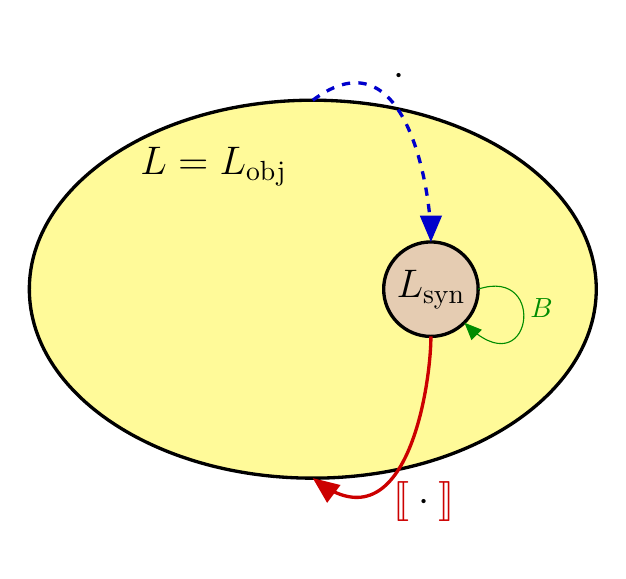
\begin{tikzpicture}[scale=.6]
  \filldraw[very thick, fill=yellow!40] (3.5,0) ellipse (6 and 4);
    \draw (+1.4,+2.6) node {\Large $L=L_{\rm obj}$};
  \filldraw[very thick, fill=brown!40] (+6,0) circle (1);
    \draw (+6,0) node {\Large $L_{\rm syn}$};
  \draw[-triangle 45, very thick, dashed, color=blue!80!black] (3.5,4) .. controls
    (5.5,5.5) and (6,2).. (6,1);
    \draw[right] (5,4.5) node {\Large $\bluesynbrack{\cdot}$};
  \draw[-triangle 45, very thick, color=red!80!black] (6,-1) .. controls
    (6,-2) and (5.5,-5.5) .. (3.5,-4);
    \draw[right] (5,-4.5) node {\Large $\redsembrack{\cdot}$};
  \draw[-triangle 45, color=green!55!black] (7,0) .. controls 
    (8.5,.5) and (8.13,-2.13) .. (6.71,-.71);
    \draw[right] (7.9,-.4) node {\bgreen{$B$}};
\end{tikzpicture}
\end{figure}
\vfill
\end{frame}

%%%%%%%%%%%%%%%%%%%%%%%%%%%%%%%%%%%%%%%%%%%%%%%%%%%%%%%%%%%%

\begin{frame}
\frametitle{Design Problems}

Several challenging \bblue{design problems} face the logic engineer
who seeks to incorporate global quotation and evaluation into a
traditional logic:

\be

  \item \bblue{Evaluation Problem}.  In a sufficiently strong theory,
    it is possible to express the liar paradox as an expression
    \mname{LIAR} that equals $\synbrack{\Neg\sembrack{\mname{LIAR}}}$
    so that

  \bi

    \item[] $\sembrack{\mname{LIAR}} =
      \sembrack{\synbrack{\Neg\sembrack{\mname{LIAR}}}} = \Neg\sembrack{\mname{LIAR}}$

  \ei

  by the law of disquotation. 

  \item \bblue{Variable Problem}.  If $c = \synbrack{x}$, then $x$ is
    free in $\sembrack{c}$ since

  \bi

    \item[] $\sembrack{c} = \sembrack{\synbrack{x}} = x$

  \ei

  by the law of disquotation.

  \item \bblue{Double Substitution Problem.}

  \item \bblue{Constant Interpretation Problem}.

\ee
\end{frame}

%%%%%%%%%%%%%%%%%%%%%%%%%%%%%%%%%%%%%%%%%%%%%%%%%%%%%%%%%%%%

\begin{frame}
\frametitle{{\churchqe}, a Version of Church's Type Theory}
\bi

  \item Based on Andrews' {\qzero}, \bblue{{\churchqe}} is a version
    of Church's type theory with a built-in global metareasoning
    infrastructure:

  \be

    \item An \bgreen{inductive type \bred{$\epsilon$} of syntactic values}
      that represent all the expressions of the logic.

    \item A partial global \bgreen{quotation operator}
      \bred{$\synbrack{\cdot}$}.

    \item A typed global \bgreen{evaluation operator}
      \bred{$\sembrack{\cdot}_\alpha$}.

  \ee

\pause

  \item {\churchqe} is the third major attempt (after \bblue{Chiron}
    and \bblue{\qzerouqe}) to develop a traditional logic with global
    quotation and evaluation.

\pause

  \item The proof system for {\churchqe} provides the ability to
    \bgreen{express}, \bgreen{prove}, and \bgreen{instantiate} schemas
    and meaning formulas.

\pause

  \item \bred{We believe {\churchqe} is the first readily
    implementable version of simple type theory with global quotation
    and evaluation.}

\ei
\end{frame}

%%%%%%%%%%%%%%%%%%%%%%%%%%%%%%%%%%%%%%%%%%%%%%%%%%%%%%%%%%%%

\begin{frame}
\frametitle{{\churchqe}: Syntax}
\bi

  \item A \bblue{expression of type $\alpha$} is inductively defined
    by the following formation rules:

  \be

    \item \bblue{Variable}: A variable $\textbf{x}_\alpha$ is an
      expression of type $\alpha$.

    \item \bblue{Constant}: A constant $\textbf{c}_\alpha$ is an
      expression of type $\alpha$.

    \item \bblue{Function application}: $(\textbf{F}_{\alpha \tarrow
      \beta} \, \textbf{A}_\alpha)$ is an expression of type $\beta$.

    \item \bblue{Function abstraction}: $(\LambdaApp \textbf{x}_\alpha
      \mdot \textbf{B}_\beta)$ is an expression of type $\alpha
      \tarrow \beta$.

    \item \bblue{Quotation}: $\synbrack{\textbf{A}_\alpha}$ is an
      expression of type $\epsilon$ if $\textbf{A}_\alpha$ is
      \bred{eval-free}.

    \item \bblue{Evaluation}: $\sembrack{\textbf{A}_\epsilon}_{{\bf
        B}_\beta}$ is an expression of type $\beta$.

  \ee 

\medskip

  \item \bred{The restriction on quotation resolves the Evaluation
    Problem!}

\ei
\end{frame}

%%%%%%%%%%%%%%%%%%%%%%%%%%%%%%%%%%%%%%%%%%%%%%%%%%%%%%%%%%%%

\begin{frame}
\frametitle{{\churchqe}: Substitution}
\bi

  \item Due to the Variable Problem, {\churchqe} requires a
    semantics-dependent form of substitution.

\pause

  \item We could introduce a logical constant \mname{sub} in {\churchqe}
    such that

  \bi

    \item[] $\mname{sub}\,\, \synbrack{\textbf{A}_\alpha} \,
      \synbrack{\textbf{x}_\alpha} \, \synbrack{\textbf{B}_\beta} =
     \synbrack{\textbf{C}_\beta}$

  \ei

  holds iff ``$\textbf{C}_\beta$ is the result of substituting
      $\textbf{A}_\alpha$ for each free occurrence of
      $\textbf{x}_\alpha$ in $\textbf{B}_\beta$ without any variable
      captures''\\ \bred{--- but this works only for eval-free expressions.}

\pause

  \item We implement substitution using Andrews' beta-reduction rules:

  \bi

    \item In the function abstraction rule we replace the
      syntactic notion of \bgreen{``a variable is \bred{free} in an
        expression''} with the more restrictive semantic notion of
      \bgreen{``a variable is \bred{effective} in an expression''}.

    \item We add rules for quotations and evaluations.

  \ei

\pause

  \item \bred{This approach resolves the Variable Problem!}

\ei
\end{frame}

%%%%%%%%%%%%%%%%%%%%%%%%%%%%%%%%%%%%%%%%%%%%%%%%%%%%%%%%%%%%

\begin{frame}
\frametitle{{\churchqe}: New Beta-Reduction Rules}
\bi

  \item \bblue{Function Abstraction Rule}

\medskip

$(\Neg \mname{IS-EFFECTIVE-IN}(\textbf{y}_\beta,\textbf{A}_\alpha)\Or
    \Neg \mname{IS-EFFECTIVE-IN}(\textbf{x}_\alpha,\textbf{B}_\gamma))
    \Implies {}$ 
\hspace*{2ex}$(\LambdaApp \textbf{x}_\alpha \mdot
    \LambdaApp \textbf{y}_\beta \mdot \textbf{B}_\gamma) \,
    \textbf{A}_\alpha = \LambdaApp \textbf{y}_\beta \mdot ((\LambdaApp
    \textbf{x}_\alpha \mdot \textbf{B}_\gamma) \,
    \textbf{A}_\alpha)$

\medskip

where $\textbf{x}_\alpha$ and $\textbf{y}_\beta$ are distinct.

\medskip

  \item \bblue{Quotation Rule}

\medskip

$(\LambdaApp \textbf{x}_\alpha \mdot \synbrack{\textbf{B}_\beta}) \,
    \textbf{A}_\alpha = \synbrack{\textbf{B}_\beta}$.

\medskip

  \item \bblue{Evaluation Rule}

\medskip

$(\mname{is-expr}_{\epsilon \tarrow o}^{\beta} \, ((\LambdaApp
    \textbf{x}_\alpha \mdot \textbf{B}_\epsilon) \, \textbf{A}_\alpha)
    \Andd {}$
\hspace*{2ex} $\Neg(\mname{is-free-in}_{\epsilon \tarrow \epsilon
  \tarrow o} \, \synbrack{\textbf{x}_\alpha} \, ((\LambdaApp
\textbf{x}_\alpha \mdot \textbf{B}_\epsilon) \, \textbf{A}_\alpha)))
\Implies {}$
\hspace*{6ex} $(\LambdaApp \textbf{x}_\alpha \mdot
\sembrack{\textbf{B}_\epsilon}_\beta) \, \textbf{A}_\alpha =
\sembrack{(\LambdaApp \textbf{x}_\alpha \mdot \textbf{B}_\epsilon) \,
  \textbf{A}_\alpha}_\beta$.

\ei
\end{frame}

%%%%%%%%%%%%%%%%%%%%%%%%%%%%%%%%%%%%%%%%%%%%%%%%%%%%%%%%%%%%

\begin{frame}
\frametitle{HOL Light QE}
\bi

  \item \bblue{HOL Light QE} is an implementation of {\churchqe}
    obtained by modifying the \bblue{HOL Light} proof assistant.

  \bi

    \item HOL Light QE is, roughly speaking, HOL Light plus global
      quasiquotation and evaluation operators.

    \item Developed by \bbrown{Patrick Laskowski} under the
      supervision of Jacques Carette and William Farmer on a summer
      undergraduate research project.

    \item It is available at

    \bi

      \item[] \href{https://github.com/JacquesCarette/hol-light-qe}
        {https://github.com/JacquesCarette/hol-light-qe}.

    \ei

  \ei

  \item Why we are using HOL Light:

  \be

    \item It is open source software.

    \item Its underlying logic is a version of Church's type theory.

    \item It provides support for defining inductive types.

  \ee

\ei
\end{frame}

%%%%%%%%%%%%%%%%%%%%%%%%%%%%%%%%%%%%%%%%%%%%%%%%%%%%%%%%%%%%

\begin{frame}
\frametitle{Implementation Stages}
\be

  \item HOL term structure is extended.

  \bi

    \item Constructors are added to the OCaml type: \bred{Quote},
      \bred{Hole}, and \bred{Eval} for building \bgreen{quotations},
      \bgreen{antiquotations}, and \bgreen{evaluations}.

    \item Inductive types of syntactic values are added for HOL Light
      QE \bgreen{types} and \bgreen{eval-free terms}.

  \ei

  \item HOL Light proof system is modified.

  \bi

    \item Rules for reasoning about quotations and evaluations.

    \item INST rule is modified to work like substitution in
      {\churchqe}.

  \ei

  \item Machinery for quotations and evaluations is created.

  \bi

    \item New functions, tactics, and theorems.

  \ei

  \item Examples are developed in the new system.

  \bi

    \item Law of Excluded Middle as a schema.

    \item Induction schemas for Presburger and Peano arithmetic.

  \ei

\ee
\end{frame}

%%%%%%%%%%%%%%%%%%%%%%%%%%%%%%%%%%%%%%%%%%%%%%%%%%%%%%%%%%%%

\begin{frame}
\frametitle{Future Work}
\bi

  \item Continue the development of HOL Light QE.

  \item Formalize simple SBMAs such as:

  \bi

    \item isEven on unary natural number numerals.

    \item Tautology checker on boolean expressions.

    \item Addition and multiplication on binary natural number
      numerals.

  \ei

  \item Formalize symbolic differentiation algorithms.

  \item Formalize a graph of biform theories encoding natural number
    arithmetic.

\ei
\end{frame}

%%%%%%%%%%%%%%%%%%%%%%%%%%%%%%%%%%%%%%%%%%%%%%%%%%%%%%%%%%%%

\begin{frame}
\frametitle{Conclusion}
\be

  \item SBMAs can be formalized using reflection.

  \item Unlike local reflection, global reflection requires only a
    single metareasoning infrastructure.

  \item {\churchqe} is a version of Church's type theory with a
    built-in global metareasoning infrastructure.

  \item HOL Light QE demonstrates that is {\churchqe} is
    implementable.

  \item Further development of HOL Light QE is needed to demonstrate
    the advantages global reflection has over local reflection.

\ee
\end{frame}

%%%%%%%%%%%%%%%%%%%%%%%%%%%%%%%%%%%%%%%%%%%%%%%%%%%%%%%%%%%%

\begin{frame}\label{lastframe}
\frametitle{References}
\bi

\footnotesize


  \item \bbrown{[And02]} P. B. Andrews, \emph{An Introduction to
    Mathematical Logic and Type Theory: To Truth through Proof, Second
    Edition}, Kluwer, 2002.

  \item \bbrown{[CarFar17]} J. Carette and W. Farmer, ``Formalizing
    Mathematical Knowledge as a Biform Theory Graph: A Case Study'',
    in: \emph{Intelligent Computer Mathematics}, LNCS 10383:9--24,
    2017.

  \item \bbrown{[Far13]} W. M. Farmer, ``The Formalization of
    Syntax-Based Mathematical Algorithms using Quotation and
    Evaluation'', in: \emph{Intelligent Computer Mathematics}, LNCS
    7961:35--50, 2013.

  \item \bbrown{[Far13a]} W. M. Farmer, ``Chiron: A Set Theory with
    Types, Undefinedness, Quotation, and Evaluation'', in: CoRR,
    abs/1305.6206 (154~pp.), 2013.

  \item \bbrown{[Far14]} W. M. Farmer, ``Simple Type Theory with Undefinedness,
    Quotation, and Evaluation'', in: CoRR,
    abs/1406.6706 (87~pp.), 2014.

  \item \bbrown{[Far17]} W. M. Farmer, ``Theory Morphisms in Church's
    Type Theory with Quotation and Evaluation'', \emph{Intelligent
      Computer Mathematics}, LNCS 10383:147--162, 2017.

  \item \bbrown{[Far18]} W. M. Farmer, ``Incorporating Quotation and
    Evaluation into Church's Type Theory'', \emph{Information and
      Computation}, 260:9--50, 2018.

\ei
\end{frame}

\iffalse

%%%%%%%%%%%%%%%%%%%%%%%%%%%%%%%%%%%%%%%%%%%%%%%%%%%%%%%%%%%%

\begin{frame}
\frametitle{}
\bi

  \item 

\ei
\end{frame}

\fi

\end{document}
